\documentclass{article}
\usepackage[utf8]{inputenc}
\PassOptionsToPackage{usenames,dvipsnames,svgnames}{xcolor}  
\usepackage{kotex}
\usepackage{verbatim}
\usepackage{graphicx}
\usepackage{indentfirst}
\usepackage{caption}
\usepackage{subcaption}
\usepackage{listings}
\usepackage{xcolor}
\usepackage{tikz}
\usetikzlibrary{arrows,positioning,automata}
\usepackage{geometry}
\usepackage{amsmath}
\usepackage{enumitem}
\usepackage{verbatim}

\renewcommand{\figurename}{그림}
\renewcommand{\tablename}{표}
\renewcommand{\contentsname}{목차}
\renewcommand{\lstlistingname}{코드}
\renewcommand{\listfigurename}{\figurename 목차}
\renewcommand{\listtablename}{\tablename 목차}
\renewcommand{\lstlistlistingname}{\lstlistingname 목차}

\geometry{
    a4paper,
    left=30mm,
    right=30mm,
    top=30mm,
    bottom=40mm
}

\lstset{language=C++,
            basicstyle=\ttfamily,
            keywordstyle=\color{blue}\ttfamily,
            stringstyle=\color{red}\ttfamily,
            commentstyle=\color{teal}\ttfamily,
            numberstyle=\tiny\color{gray}\ttfamily,
            morecomment=[l][\color{magenta}]{\#}
            breakatwhitespace=false,         
            breaklines=true,                 
            captionpos=b,                    
            keepspaces=true,                 
            numbers=left,                    
            numbersep=5pt,                  
            showspaces=false,                
            showstringspaces=false,
            showtabs=false,                  
            tabsize=2
}

\title{DataStructure HW10}
\author{C211123 이준선}
\date{December 2022}

\begin{document}

\maketitle
\tableofcontents
\listoffigures
\lstlistoflistings
\thispagestyle{empty}
\newpage

\pagenumbering{arabic}
\section{개요}
지하철의 노선도를 입력받고, 시작역과 도착역을 입력받아 두 역 사이의 최소 시간 경로와 두 역 간 이동 시간의 차이가 최소가 되게 하는 중간역을 출력하는 프로그램을 작성하였다. 지하철의 노선도는 ``호선 출발역 호선 도착역" 형태의 파일 구조로 되어 있고, 시작역과 도착역 역시 마찬가지이다. 한편 중간역이라 함은 시작역에서 중간역까지 걸리는 시간, 도착역에서 중간역까지 걸리는 시간의 차이가 최소가 되게 하는 역을 의미한다. 모든 역간 이동 시간은 60초이며, 호선이 바뀌는 환승역에서는 30초가 추가된다.

\section{문제 구성}
\subsection{문제}
\begin{enumerate} [label=(\alph*)]
    \item 준회(출발역)는 현수네 집(도착역)에 지하철을 타고 가기로 했다. 이때 최소 시간 경로 및 걸리는 시간을 구하여라.
    \item 현수가 생각해보니 본인의 집이 더럽다며 그냥 밖에서 만나자고 했다. 이때 각자 걸리는 시간의 차이가 최소가 되는 역과 시간을 구하여라.
\end{enumerate}

\subsection{입력 파일}
문제에서 사용된 입력 파일은 역간 정보를 구성하는 stations1.txt 파일과 출발역과 도착역 정보를 담고 있는 input1.txt 파일이다.

station1.txt 파일은 다음과 같이 구성되어 있다.
\begin{itemize}
    \item 첫 줄의 경우 총 역의 개수이다. 예를 들어 72면, 72개의 역 정보가 있다는 의미이다.
    \item 둘 째줄부터 역 정보가 구성되어 있다.\\
    띄어쓰기를 기준으로 (출발역의 호선) (출발역) (도착역의 호선) (도착역) 순으로 정보가 구성되어 있다. 출발역$\longleftrightarrow$도착역 간 양방향으로 직접 연결되어 있다는 의미이다. 예를 들어 다음과 같이 구성되어 있다: \\
    1 Jongno$\_$5(o)-ga 1 Jongno\_3(sam)-ga \\
    1 Jongno\_3(sam)-ga 1 Jonggak \\
    1 Jonggak 1 City\_Hall \\
    1 City\_Hall 1 Seoul\_Station\\
    1 Seoul\_Station 1 Namyeong\\
    1 Namyeong 1 Yongsan\\
    1 Yongsan 1 Noryangjin\\
    1 Noryangjin 1 Daebang
    
    \item 만약 환승역의 경우, (환승 전의 호선) (환승역) (환승 후의 호선) (환승역) 순으로 정보가 구성되어 있을 수도 있다. 예를 들어 다음과 같이 구성되어 있다:\\
    1 City\_Hall 2 City\_Hall\\
    그러나 모든 환승역이 위와 같이 구성되어 있는 것은 아니며, station1.txt의 경우 1호선과 2호선을 잇는 환승역인 신도림의 경우 다음과 같이 구성되어 있다:\\
    1 Yeongdeungpo 1 Sindorim \\
    1 Sindorim 1 Guro \\
    $\vdots$ \\
    2 Daerim 2 Sindorim\\
    2 Sindorim 2 Mullae
    
    \item 역 이름에는 띄어쓰기가 없다. 
    \item 한글 이름의 역은 존재하지 않는다.
    \item 실제 2호선처럼 순환하는 호선이 있을 수 있다.
    \item 실제 1호선처럼 나뉘는 호선이 있을 수 있다.
    \item 호선의 개수는 1 이상 9 이하의 자연수이다\footnote{1호선부터 9호선을 의미하며, 인천1호선, 수인선과 같은 호선은 고려하지 않는다.}.
    \item 모든 역은 양방향을 오갈 수 있어야 한다.
\end{itemize}

input1.txt 파일은 다음과 같이 구성되어 있다.
\begin{itemize}
    \item 첫 줄은 출발역, 둘 째줄은 도착역의 정보가 입력되어 있다. 역 정보는 stations1.txt와 같이 띄어쓰기를 기준으로 (출발역의 호선) (출발역) (도착역의 호선) (도착역) 순으로 정보가 구성되어 있다. 예를 들어 다음과 같이 구성되어 있다:\\
    3 Anguk\\
    2 Chungjeongno
\end{itemize}

각 역간 이동은 순차적으로만 이동 가능하며, 노선의 변경은 환승역을 이용해야 한다. 각 역간 이동 시간은 60초, 환승 시간은 30초가 추가된다.

\subsection{입력 받기}
\begin{lstlisting} [language=C++, escapeinside=``, caption=main.cpp, label={lstlinsting:readFile_main.cpp}]
int main(int argc, char* argv[])
{
	int numLine;
	int line1, line2;
	string src, dst;
	if (argc != 3) {
		cerr << "Argument Count is" << argc << endl << "Argument must be " <<
			argc << endl;
		return 1;
	}
	fstream fin(argv[1]);
	if (!fin) {
		cerr << argv[1] << " open failed" << endl;
		return 1;
	}
	fin >> numLine;
	
	Subway subway;
	// read file and insert station
	for (int i = 0; i < numLine; i++) {
		int line1, line2; // line1 = line of src, line2 =line of dst
		string src, dst;
		fin >> line1 >> src >> line2 >> dst;

		subway.make_station(src, line1, dst, line2);
	}
	fin.close();

	// input1.txt `시작역과 도착역 정보 읽기`
	fstream fin2(argv[2]);
	if (!fin2) {
		cerr << argv[2] << " open failed" << endl;
		return 1;
	}
	fin2 >> line1 >> src; // start(source) station
	fin2 >> line2 >> dst; // destination station
	fin2.close();
 
	return 0;
}
\end{lstlisting}

코드 \ref{lstlinsting:readFile_main.cpp}은 stations1.txt와 input1.txt를 입력받는 main함수를 나타낸 것이다\footnote{main.cpp의 전문이 아니며, 입력받는 부분만 표시되었다.}. Subway 클래스는 지하철 경로 탐색 등에 필요한 함수들과 변수들이 저장된 클래스이다. Subway 타입의 subway를 생성한 뒤, 역 정보를 make\_station 함수에 전달해 그래프를 전달한다.

\begin{lstlisting} [language=C++, escapeinside=``, caption={make\_station function}, label={lstlinsting:add_connection}]
void Subway::make_station(string src, int line1, string dst, int line2)
{
	insert_station(src);
	insert_station(dst);

	// add connection
	add_connection(src, dst, line1, line2);
}
\end{lstlisting}

코드 \ref{lstlinsting:add_connection}은 make\_station 함수로, insert\_station 함수로 src(출발역)과 dst(도착역)을 생성하고, add\_connection 함수로 src와 dst를 연결한다.

\subsection{그래프 구성 방식}
\begin{lstlisting}[language=C++, escapeinside=``, caption={subway.h 그래프 형성}, label={lstlinsting:subway.h graph making}]
class Station {
public:
	string name;
	vector<Connector*> connections;
	int max_time;
	Station(string name);
	friend ostream& operator<<(ostream& os, const Station& station);
};

class Connector {
public:
	Station* dst;
	int line;
	int distance;
	Connector(Station* dst, int line, int distance);
};

class Subway {
private:
	map<string, Station*> station_list;
};
\end{lstlisting}

\begin{lstlisting} [language=C++, escapeinside=``, caption={insert\_station and add\_connection function}, label={lstlinsting:insert and add function}]
// function that insert a station into the station_list
void Subway::insert_station(string name) {
	Station* station = new Station(name);
	station_list.insert(pair<string, Station*>(name, station));
}

// function that add a connection between two stations
void Subway::add_connection(string src, string dst, int line1, int line2) {
	
	Station* station1 = station_list[src];
	Station* station2 = station_list[dst];
	int distance = 60; // basic distance

	// when trasfering, distance = 30
	if (src == dst && line1 != line2) {
		distance = 30;
	}
	else if (src == dst && line1 == line2) {
		string error = "Error: " + src + " and " + dst + " are the same station, but the same line";
		throw error;
	}
	
	Connector* connector1 = new Connector(station2, line1, distance);
	Connector* connector2 = new Connector(station1, line2, distance);
	station1->connections.push_back(connector1);
	station2->connections.push_back(connector2);
}
\end{lstlisting}

코드 \ref{lstlinsting:subway.h graph making}는 그래프 구성에 필요한 Station, Connector 클래스 전체와 Subway 클래스 속 map$<$string, Station*$>$ station\_list을 보여준다. 코드 \ref{lstlinsting:insert and add function}는 그래프를 형성하는 중요한 두 함수인 insert\_station, add\_connection 함수를 보여준다.

먼저 클래스 Station은 역의 정보를 담는 클래스로, 다음과 같이 구성된다:
\begin{itemize}
    \item 역 이름 name
    \item 연결된 다른 역 Connections\\
    이때 Connections는 클래스 Connector를 이용해 정보를 저장한다.
    \item 역까지 이동하는데 걸리는 최대 시간. 기본적으론 10000\footnote{임의의 큰 값이며, 처음 들어온 값에 대해 무조건 갱신되게끔 하는 값이다. 만약 최소 시간이 10000이 넘어갈 경우, 이 초기값은 충분히 더 큰 값으로 갱신해야 한다.}으로 초기화하며, 만약 max\_time보다 작은 time으로 해당 역까지 이동할 수 있다면 최단 경로와 최단 시간을 갱신한다.
\end{itemize}

클래스 Connector는 한 역에 연결된 다른 역의 정보를 담는 클래스로, 다음과 같이 구성된다:
\begin{itemize}
    \item 목적지 dst
    \item 목적지의 호선 정보 line
    \item 목적지까지의 거리 정보 distance, 기본적으론 60초이나 환승역의 경우 30초이다. 한편 환승역의 경우, src와 dst가 같고 호선 정보가 다르면 환승역이라 간주한다.
\end{itemize}

station\_list는 역 리스트로, 역 이름을 키로, 역 정보가 담긴 Station 구조체가 value로 담긴 map이다. 역 이름 string으로 Station 구조체 정보를 빠르게 찾기 위한 map이다.

한편 그래프를 구성하는 방식은, Station의 connections에 Connector 정보를 추가하는 식으로 그래프를 구성한다. Connectors는 vector$<$Connector*$>$ 타입으로, 구조체 Connector의 정보를 담는다. 예를 들어 신도림 역 Shindorim Station이 다음과 같이 구성되어 있다고 하자.

Station Shindorim:
\begin{itemize}
    \item name = `Shindorim'
    \item connections = 
    \begin{itemize}
        \item Yeongdeungpo, line1, 60
        \item Guro, line1, 60
        \item Daerim, line2, 60
        \item Mullae, line2, 60
    \end{itemize}
    \item max\_time = 10000
\end{itemize}

이는 Shindorim Station이 1호선 Yeongdeungpo Station과 60초 간격만큼, 1호선 Guro Station과 60초 간격만큼, 2호선 Daerim Station과 60초 간격만큼, $\cdots$ 연결되어 있다는 의미이다. 즉 Shindorim에서 Yeongdeungpo, Guro, Daerim, Mullae 역을 갈 수 있다. 당연히 모든 역은 양방향이기에, Guro 역의 connections에도 Shindorim, line1, 60이 포함되어 있다.

함수 insert\_station은 Station 구조체를 형성한다. 역 이름을 매개 변수로 받아서, Station 구조체를 new로 동적 생성하고, 이를 station\_list에 이름과 페어를 이루어 추가한다. 이러면 station\_list[역이름]을 통해 그 역의 Station 구조체를 바로 검색할 수 있다.

함수 add\_connection은 src, dst, line1, line2를 전달받는다. line1 src $\longleftrightarrow$ line2 dst 를 형성한다. 한편 동일한 역에 대해 호선만 다르게 입력될 수 있다\footnote{$\text{src}==\text{dst}$이나 $\text{line1}\neq\text{line2}$인 경우}. 이때는 시간 정보인 distance\footnote{가중치를 의미. distance는 거리 정보를 의미하는 단어이나 여기서는 시간과 거리가 같은 가중치를 가지기에 같은 의미로 사용한다.}를 60이 아닌 30으로 놓고 역을 추가한다. 즉 호선이 다른 경우 같은 이름의 역에 대해서도 Connector를 가질 수 있다.
\begin{lstlisting} [language=C++]
Connector* connector1 = new Connector(station2, line1, distance);
Connector* connector2 = new Connector(station1, line2, distance);
station1->connections.push_back(connector1);
station2->connections.push_back(connector2);
\end{lstlisting}
이 부분이 각각 line1 src $\rightarrow$ line2 dst와 line2 dst $\rightarrow$ line1 src를 형성하는 코드이다. 양방향으로 Connector를 놓는다. 이 함수들을 이용해서 코드 \ref{lstlinsting:add_connection}에서 역간 그래프를 추가한다.

\section{(a) 최소 시간 경로 찾기}
\subsection{다익스트라 알고리즘 선택 이유}
\begin{figure}
\begin{subfigure} {0.5\textwidth}
    \centering
    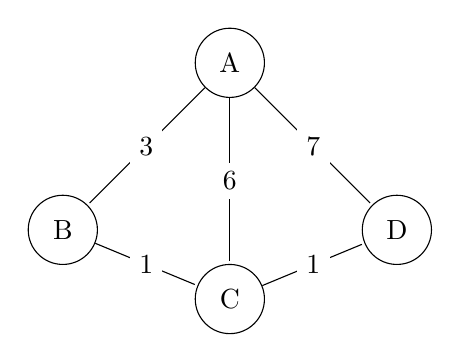
\begin{tikzpicture}[>=stealth',shorten >=1pt,node distance=3cm,on grid,initial/.style    ={}]
        \node[state] (1) {A}; 
        \node[state] (2) [below left of=1] {B}; 
        \node[state] (3) [below of=1] {C}; 
        \node[state] (4) [below right of=1] {D};
        \tikzset{every node/.style={fill=white}}
        \path   (1) edge node {$3$} (2)
                (1) edge node {$6$} (3)
                (1) edge node {$7$} (4)
                (2) edge node {$1$} (3)
                (3) edge node {$1$} (4); 
    \end{tikzpicture}
    \caption{과정 1, 초기 상태}
    \label{fig:graph_1}
\end{subfigure}
\hfill
\begin{subfigure} {0.5\textwidth}
    \centering
    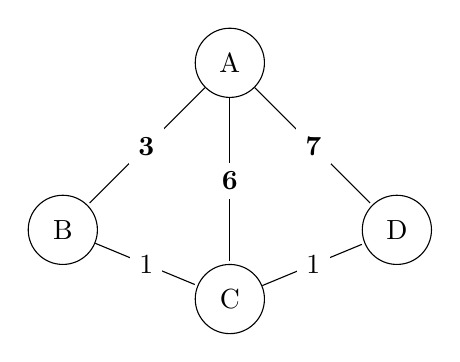
\begin{tikzpicture}[>=stealth',shorten >=1pt,node distance=3cm,on grid,initial/.style    ={}]
        \node[state] (1) {A}; 
        \node[state] (2) [below left of=1] {B}; 
        \node[state] (3) [below of=1] {C}; 
        \node[state] (4) [below right of=1] {D};
        \tikzset{mystyle/.style={-, double=black}}
        \tikzset{every node/.style={fill=white}}
        \path   (2) edge node[mystyle] {$1$} (3)
                (3) edge node[mystyle] {$1$} (4); 
        \tikzset{mystyle/.style={-, double=blue}} 
        \path   (1) edge node[mystyle] {$\textbf{3}$} (2)
                (1) edge node[mystyle] {$\textbf{6}$} (3)
                (1) edge node[mystyle] {$\textbf{7}$} (4);
    \end{tikzpicture}
    \caption{과정 2}
    \label{fig:graph_2}
\end{subfigure}
\vfill
\begin{subfigure} {0.5\textwidth}
    \centering
    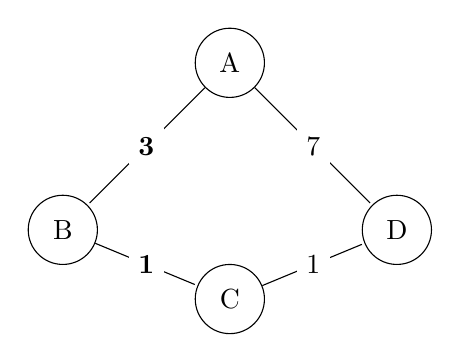
\begin{tikzpicture}[>=stealth',shorten >=1pt,node distance=3cm,on grid,initial/.style    ={}]
        \node[state] (1) {A}; 
        \node[state] (2) [below left of=1] {B}; 
        \node[state] (3) [below of=1] {C}; 
        \node[state] (4) [below right of=1] {D};
        \tikzset{every node/.style={fill=white}}
        \path   (1) edge node {$\textbf{3}$} (2)
                (1) edge node {$7$} (4)
                (2) edge node {$\textbf{1}$} (3)
                (3) edge node {$1$} (4); 
    \end{tikzpicture}
    \caption{과정 3}
    \label{fig:graph_3}
\end{subfigure}
\hfill
\begin{subfigure} {0.5\textwidth}
    \centering
    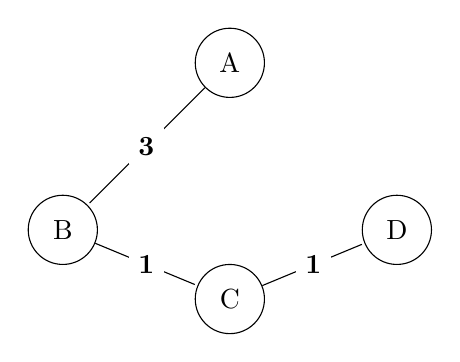
\begin{tikzpicture}[>=stealth',shorten >=1pt,node distance=3cm,on grid,initial/.style    ={}]
        \node[state] (1) {A}; 
        \node[state] (2) [below left of=1] {B}; 
        \node[state] (3) [below of=1] {C}; 
        \node[state] (4) [below right of=1] {D};
        \tikzset{every node/.style={fill=white}}
        \path   (1) edge node {$\textbf{3}$} (2)
                (2) edge node {$\textbf{1}$} (3)
                (3) edge node {$\textbf{1}$} (4); 
    \end{tikzpicture}
    \caption{과정 4, 최종 상태}
    \label{fig:graph_4}
\end{subfigure}
\caption{다익스트라의 최단 경로 생성 과정}
\label{graph_whole}
\end{figure}

최단 경로 찾기에는 DFS, BFS, 다익스트라(Dijkstra), A*, $\theta$* 알고리즘 등 다양한 알고리즘이 존재한다. 각각의 알고리즘들은 각각의 상황과 경우에 맞추어 적합하다. 예를 들어 BFS는 거리, 시간 등의 가중치가 부여되지 않는 경우에 최단 경로를 찾기 유리하며, A* 알고리즘은 휴리스틱 기법을 도입해 성능을 크게 향상시킨 경로 찾기 알고리즘으로, 휴리스틱 기법을 적용할 수 있는 현실 세계의 지도나 실제 게임 지도 상에서의 경로 찾기에 유리하다. $\theta$* 알고리즘은 기계적인 움직임을 보이는 A* 알고리즘 경로를 자연스러운 시각 정보를 반영하여 부드럽게 움직일 수 있게 해주는 경로 스무딩 알고리즘으로, 기계적인 최단 경로를 찾아가는 것보다 캐릭터의 자연스러운 움직임을 구현하는데 중요한 게임 속에서 자주 사용한다. 한편 이 문제의 경우, 지하철 노선에 대한 정보만 존재하여 휴리스틱을 구현하기 힘들고, 각 역간 이동 시간과 환승 시간이라는 가중치가 존재한다. 이 경우 \textbf{다익스트라 알고리즘}이 가장 적합한 알고리즘일 것이다.

다익스트라 알고리즘은 음의 가중치가 없는 그래프에서 한 정점과 다른 모든 정점 사이의 최단 경로를 구하는 탐욕적 방법의 알고리즘으로, 실제 음의 가중치를 갖는 경우는 매우 드물기에 널리 사용되는 기법의 알고리즘이다. 각 간선간 가중치가 모두 다를 때 유리하며, 우선순위 큐(힙)을 사용할 경우 최악의 시간 복잡도가 $\textit{O}(n\log{n})$임을 보장한다. 단, 이번 문제에서는 각 역간 이동 시간이 모두 60초로 동일한 점, 그리고 환승 시에만 환승 시간 30초가 추가된다는 점, 한 정점(Vertex)이 3개 이상의 간선(Edge)를 갖는 경우가 극히 드물다는 점을 고려하여, 우선순위 큐를 사용해도 큰 폭의 성능 향상을 기대할 수 없을 거란 판단에 하에 구현 난이도가 높은 우선순위 큐의 사용을 하지 아니하였다. 이럴 경우 훨씬 직관적인 코드 구성이 가능하다\footnote{단 이럴 경우 최악의 시간 복잡도가 $\textit{O}(n)$인 단점이 있으나, 문제 조건 상 역의 개수가 한 호선 당 최대 100개씩 900개로 제한되어 있어, 큰 문제는 아닐 것이라 판단된다.}.

한편 다익스트라 알고리즘의 기본 전제는 `최단 경로는 여러 개의 최단 경로로 이루어져 있다'라는 것이다. 즉 만약 정점 A에서 정점 D까지 가는 최단 경로가 A$\rightarrow$B$\rightarrow$C$\rightarrow$D라면, 경로 A$\rightarrow$B, B$\rightarrow$C, A$\rightarrow$B$\rightarrow$C, B$\rightarrow$C$\rightarrow$D도 모두 최단 경로일 것이라 가정하는 것이다. 물론 위 경우와 맞지 않는 특수한 경우를 반례로 구성할 경우, 위 가정은 거짓이 되므로 다익스트라에서 구한 최단 경로가 수학적으로 실제 최단 경로임을 보장하지는 않는다. 그러나 그리디 알고리즘의 특성상 수학적으로 참인 해를 보장하진 않지만 참에 가까운 해를 빠른 시간 복잡도로 구할 수 있다는 장점이 있다.

다익스트라 알고리즘의 작동 과정은 다음과 같다:
\begin{enumerate}
    \item 출발 노드를 설정합니다.
    \item 출발 노드를 기준으로 각 노드의 최소 비용을 저장합니다.
    \item 방문하지 않은 노드 중에서 가장 비용이 적은 노드를 선택합니다.
    \item 해당 노드를 거쳐서 특정한 노드로 가는 경우를 고려하여 최소 비용을 갱신합니다.
    \item 위 과정에서 3번, 4번을 반복합니다.
\end{enumerate}

그림 \ref{fig:graph_1}에서 정점 A를 보면, 현재 A에서 B, C, D로 가는 비용은 3, 6, 7로 확인할 수 있다(그림 \ref{fig:graph_2}). 그러나 정점 B에 대해 처리하면, 경로 A$\rightarrow$B$\rightarrow$C의 비용이 4로 경로 A$\rightarrow$C의 6보다 더 작다는 것을 알 수 있다. 이때 A에서 C로 가는 최단 경로를 A$\rightarrow$B$\rightarrow$C로 새롭게 갱신하고, A$\rightarrow$C를 무시하는 것이다(그림 \ref{fig:graph_3}). 마찬가지로 노드 C에 대해 각 최소 경로를 확인하면, A에서 D로 가는 최단 경로가 A$\rightarrow$B$\rightarrow$C$\rightarrow$D 임을 알 수 있고, 이때 A$\rightarrow$D를 무시한다(그림 \ref{fig:graph_4}).
\subsection{코드 구현}
\begin{lstlisting} [language=C++, escapeinside=``, caption={main:find\_shortest\_path}, label={lstlinsting:find shortest path public}]
void Subway::find_shortest_path(const string src, const string dst, const int line)
{
	// if src or dst are not in the station_list, throw an error
	if (station_list.find(src) == station_list.end()) {
		string error = "Error: " + src + "is not in the station_list";
		throw error;
	}
	else if (station_list.find(dst) == station_list.end()) {
		string error = "Error: " + dst + "is not in the station_list";
		throw error;
	}
	
	vector<Station*> path;
	try {
		find_shortest_path(path, src, dst, line, 0);
	}
	catch (string error) {
		std::cout << error << std::endl;
	}
	print_shortest_path();
}

// dir_list `중 가장 짧은 시간을 가진 경로를 출력`
void Subway::print_shortest_path()
{
	set_shortest_path();
	
	std::cout << "Shortest path : " << endl;
	print_path(min_path);

	int minute = min_time / 60;
	int seconds = min_time % 60;
	std::cout << "Time : " << minute << " min " << seconds << " sec" << " (" << min_time << " seconds)" << endl;
}

void Subway::set_shortest_path()
{
	int min_time = 10000;
	int min_index = 0;
	for (int i = 0; i < dir_list.size(); i++) {
		if (dir_list[i].second < min_time) {
			min_time = dir_list[i].second;
			min_index = i;
		}
	}

	// min_path`에 최소 경로 저장`
	min_path = dir_list[min_index].first;
	this->min_time = dir_list[min_index].second;
}
\end{lstlisting}

코드 \ref{lstlinsting:find shortest path public}에서 find\_shortest\_path는 public하게 접근할 수 있지만, 실제 다익스트라 알고리즘을 사용하여 최단 경로를 찾는 동명의 함수는 private하게 숨겨져 있다. 이 이유는 후에 `class 설계 내용 및 이유' 파트에서 다룬다.

public find\_shortest\_path 함수에서 먼저 src, dst가 station\_list에 존재하는지 확인하고, 빈 Station 벡터 리스트 path를 생성한다. 이 path는 deep copy로 private find\_shortest\_path로 전달된다. 이 path에 경로가 저장된다.

private find\_shortest\_path에서 list\_dir에 path정보를 저장할 것이다. 이때 주의할 점은, private find\_shortest\_path는 src == dst인 모든 path를 저장할 수도 있다는 것이다. 이때 list\_dir 중 가장 짧은 시간을 갖고 있는 path가 최단 경로이다.

print\_shortest\_path() 함수는 list\_dir 중 최단 경로를 출력하는 함수이다. set\_shortest\_path 함수를 통해 list\_dir 중에서 최단 경로와 최소 시간을 각각 min\_path와 min\_time에 저장하고, 이를 출력한다.

\begin{lstlisting}[language=C++, escapeinside=``, caption={다익스트라 알고리즘 구현}, label={lstlinsting:dijkstra algorithm code}]
// station_dir : `현재까지 지나온 경로`
// current : `현재 위치`
// dst : `목적지`(destination)
// current_line : `현재 경유중인 노선` (line)
// time : `현재까지 걸린 시간` (`기본은` 0)
void Subway::find_shortest_path(vector<Station*> station_dir, string current, string dst, int current_line, int time = 0)
{
	// If the time that comes in is smaller than the max_time of the current, change the max_time of the current station to time.
	if (time < station_list[current]->max_time) {
		station_list[current]->max_time = time;
		// add current station to station_dir
		station_dir.push_back(station_list[current]);
	}
	else {
		// `새로 들어온` time`이` current`의` max_time`보다 크거나 같은 경우, 더 이상 진행하지 않는다.`
		return;
	}
	
	// `만약` current`가 `dst`와 같은 경우`, station_dir`와` time`을 `dir_list`에 추가한다.`
	if (current == dst) {
		dir_list.push_back(make_pair(station_dir, time));
		return;
	}
	
	for (int i = 0; i < station_list[current]->connections.size(); i++) {
		Connector* station = station_list[current]->connections[i];
		// transfer time : basically 0, but when transfering, it takes 30 seconds
		// when the line of current and next station is different, it is a transfer station
		int transfer_time = 0;
		if (current_line != station->line) {
			transfer_time = 30;
		}
		
		string next_station = station->dst->name;
		int next_line = station->line;
		int totalTime = time + station->distance + transfer_time;

		// `현재 위치에서 갈 수 있는 모든` station`에 대해 재귀적으로` find_shortest_path`를 호출한다.`
		// we have to pass station_dir by deep copy
		find_shortest_path(station_dir, next_station, dst, next_line, totalTime);
	}
}
\end{lstlisting}

코드 \ref{lstlinsting:dijkstra algorithm code}의 함수가 다익스트라 알고리즘을 구성하는 단 하나의 함수이다. find\_shortest\_path 함수는 매개 변수로 다음을 전달받는다:
\begin{itemize}
    \item station\_dir : 현재까지 지나온 경로
    \item current : 현재 역 이름\footnote{출발역인 src가 아님에 주의한다.}
    \item dst : 목적지
    \item current\_line : 현재 역의 호선
    \item time : 현재까지 걸린 총 시간
\end{itemize}

먼저 들어온 총 시간 time에 대해 현재 max\_time보다 작다면, 더 짧은 시간으로 max\_time을 교체하며, station\_dir에 현재 역을 추가한다. 이로써 다익스트라의 핵심 논리 중 하나인 더 짧은 정점에 대해 경로를 구성하고, 더 긴 경로는 버린다는 논리를 가질 수 있다. 한편 max\_time의 초기값은 10000으로 설정되어 있기에 처음 들어온 time에 대해서는 무조건 바뀌게 될 것이다.

한편 새로 들어온 time이 기존 max\_time보다 크다면, 그것은 이미 최소 시간을 가지는 최단 경로가 아니란 뜻이다. 따라서 그 경로는 죽은 경로(가망이 없는 노드)가 되며, 해당 경로에 대한 탐색은 더 이상 진행하지 않고 버린다.

만약 경로 탐색을 하다 current와 dst가 같은 경우, 하나의 경로를 찾은 것이다. 전체 경로를 담는 dir\_list에 지금까지 탐색한 경로 station\_dir와 총 시간을 추가한다. 그러나 이 station\_dir가 최소 시간 경로라는 의미는 아니다. 탐색을 더 하다 보면 더 짧은 경로를 찾을 수 있다.

\begin{lstlisting} [language=C++, escapeinside=``, caption={코드 \ref{lstlinsting:dijkstra algorithm code} 중 핵심 로직 확대}, label={lstlinsting:dijkstra algorithm code_recursive part}]
for (int i = 0; i < station_list[current]->connections.size(); i++) {
		Connector* station = station_list[current]->connections[i];
		// transfer time : basically 0, but when transfering, it takes 30 seconds
		// when the line of current and next station is different, it is a transfer station
		int transfer_time = 0;
		if (current_line != station->line) {
			transfer_time = 30;
		}
		
		string next_station = station->dst->name;
		int next_line = station->line;
		int totalTime = time + station->distance + transfer_time;

		// `현재 위치에서 갈 수 있는 모든` station`에 대해 재귀적으로` find_shortest_path`를 호출한다.`
		// we have to pass station_dir by deep copy
		find_shortest_path(station_dir, next_station, dst, next_line, totalTime);
	}
\end{lstlisting}
코드 \ref{lstlinsting:dijkstra algorithm code_recursive part}은 코드 \ref{lstlinsting:dijkstra algorithm code}의 재귀호출문을 확대한 것이다. 이 부분이 다익스트라 알고리즘의 핵심이 된다. 

현재 정점 current station의 모든 connection에 대해 다음 탐색을 수행한다.
\begin{enumerate}
    \item 환승 시간에 대한 정보 transfer\_time을 추가한다. transfer\_time은 기본적으론 0이지만, 환승역일 시 30이 된다.
    \item 전체 시간 totalTime = time(인자로 전달된 지금까지의 시간) + station-$>$distance(다음 역까지의 거리) + transfer\_time(환승 시간)이다.
    \item station은 connector, 즉 다음 역이다. 다음 역에 대해 find\_shortest\_path 함수를 재귀 호출한다. 이때 인자로 현재까지의 경로 정보 station\_dir와 다음 역 정보, 목적지, 다음 호선, 전체 시간을 전달한다. 주의할 점은 계속해서 강조하듯이 station\_dir은 deep copy로 전달되어야 한다. 만약 참조 형식과 같이 shallow copy로 전달될 경우 경로 정보가 꼬일 수 있다.
\end{enumerate}

한편 구현 과정 특성상 find\_shortest\_path가 재귀적으로 탐색하면서, 두 개 이상의 src와 dst를 잇는 경로를 발견할 수 있다. 때문에 발견된 모든 경로를 dir\_list에 저장하여, 위에서 설명한 과정을 통해 최단 경로를 확정하는 별도의 과정이 필요하다.

\section{(b) 중간역 찾기}
여기서 중간역이란, 시작역에서 중간역까지 걸리는 시간, 도착역에서 중간역까지 걸리는 시간의 차이가 최소가 되게 하는 역을 의미한다. 이때 중간역은 모든 역에 대해 조사할 필요는 없다. 이미 다익스트라 알고리즘을 통해 min\_path를 찾았고, 최단 경로는 여러 개의 최단 경로로 구성되어 있다\footnote{A에서 D까지 최단 경로가 A$\rightarrow$B$\rightarrow$C$\rightarrow$D라면, 경로 A$\rightarrow$B, B$\rightarrow$C, A$\rightarrow$B$\rightarrow$C, B$\rightarrow$C$\rightarrow$D도 모두 최단 경로, 위에서 선술한 내용 참고}는 가정에 따라 중간역 M에 대해 식 (\ref{eq:middleStation_M})이 성립한다.
\begin{equation}
\label{eq:middleStation_M}
    M\in\text{min\_path} \text{ s.t. } \min{\mid T_{src-M}-T_{dst-M} \mid}
\end{equation}

따라서 min\_path의 역에 대해서만 각자 걸리는 시간의 차이가 최소가 되는 역을 찾으면 된다.
\begin{lstlisting}[language=C++, escapeinside=``, caption={중간역 찾기}, label={lstlinsting:find_middle_station}]
// min_path`의 역 중에서`, src`와` dst`까지의 거리의 차가 가장 짧은, 중간 지점의 역을 찾아서 출력`
void Subway::find_middle_station(string src, string dst)
{
	if (min_path.size() == 0) {
		std::cout << "ERROR : There is no path between " << src << " and " << dst << endl;
		return;
	}
	
	Station* src_station = station_list[src];
	Station* dst_station = station_list[dst];
	int min_distance = 10000;
	Station* min_station = min_path[0];
	
	int time_src = 0;
	int time_dst = 0;
	
	for (int i = 0; i < min_path.size(); i++) {
		if (min_path[i] == src_station || min_path[i] == dst_station) {
			continue;
		}
		
		// find stations that has the smallest absolete value of the difference 
		// between the distance from src and dst
		int distance = abs(abs(min_path[i]->max_time - src_station->max_time) 
			- abs(min_path[i]->max_time - dst_station->max_time));
		if (distance < min_distance) {
			min_distance = distance;
			min_station = min_path[i];
			time_src = abs(min_path[i]->max_time - src_station->max_time);
			time_dst = abs(min_path[i]->max_time - dst_station->max_time);
		}
	}
	

	std::cout << "Middle station : " << min_station->name << endl;
	std::cout << src << " - " << min_station->name << " time : " 
		<< time_src / 60 << " min " << time_src % 60 << " sec (" 
		<< time_src << " seconds)" << endl;
	std::cout << dst << " - " << min_station->name << " time : " 
		<< time_dst / 60 << " min " << time_dst % 60 << " sec (" 
		<< time_dst << " seconds)" << endl;
	std::cout << "The difference in time taken : " << abs(time_src - time_dst) << " seconds" << endl;
}
\end{lstlisting}

코드 \ref{lstlinsting:find_middle_station}은 위에서 설명한 과정을 그대로 구현한 것이다. 최소 시간 차이를 나타내는 min\_distance\footnote{계속해서 강조하지만, 이 문제에서 시간과 거리는 사실상 같은 의미로 사용되었다.}보다 짧은 시간이 발견되면 그 값으로 갱신한다\footnote{초기값은 10000으로 설정하여 처음 한 번은 무조건 갱신되게끔 함}.

한편 중간역은 적어도 출발역이나 종착역에 있지는 않을 것이므로, 이에 대한 비교는 수행하지 않는다.

\section{클래스 설계 내용 및 이유}
\begin{lstlisting} [language=C++, escapeinside=``, caption={subway.h 클래스 설계 부분}, label={lstlinsting:subway.h class}]
class Station {
public:
	string name;
	vector<Connector*> connections;
	int max_time;
	Station(string name);
	friend ostream& operator<<(ostream& os, const Station& station);
	void printStationInfo();
	~Station();
};

class Connector {
public:
	Station* dst;
	int line;
	int distance;
	Connector(Station* dst, int line, int distance);
	void printConnectorInfo();
};

class Subway {
private:
	map<string, Station*> station_list;
	// vector<Station*> `의 벡터 리스트와` int `시간 정보의 페어`
	vector< pair<vector<Station*>, int> > dir_list;
	// `최소 경로와 시간`
	vector<Station*> min_path;
	int min_time;

	void set_shortest_path();
	void find_shortest_path(vector<Station*> station_dir, string current, string dst, int current_line, int time);
	void print_path(vector<Station*> path);
	void insert_station(string name);
	void add_connection(string src, string dst, int line1, int line2);
public:
	void make_station(string src, int line1, string dst, int line2);
	void print_shortest_path();
	void find_shortest_path(const string src, const string dst, const int line);

	// src`와` dst `사이에 걸리는 시간의 차이가 최소가 되는` middle station`을 찾는 함수`
	void find_middle_station(string src, string dst);

	void print_station_info(string name);
	void printAllStations();
	~Subway();
};
\end{lstlisting}

프로그램은 사용자에게 간단한 인터페이스를 제공하는 한편, 접근하기에 위험할 수 있는 정보들을 차단하는 방식으로 설계되었다.

먼저 Station과 Connector은 사실상 구조체 struct처럼 사용한다. 각각의 정보를 출력하는 printConnectorInfo 함수와 printStationInfo가 존재한다.

사용자가 주로 사용하는 클래스는 Subway 클래스이다. station\_list, dir\_list, min\_path, min\_time은 민감한 내부 정보이므로 보호한다. 사용자는 이 정보에 오직 public 함수를 통해서만 간접적으로 접근할 수 있다. 정보를 가리고 접근을 제한하는 이유는 객체 지향 프로그래밍(OOP)의 기본 설계 원칙이므로 추가적인 설명은 생략한다.

한편 set\_shortest\_path, find\_shortest\_path는 public한 find\_shortest\_path에서 내부적으로 사용한다. 일반 사용자는 접근할 일이 없는 함수들이고, private한 변수들에 접근하므로 private로 분류하였다. insert\_station, add\_connection 함수 역시 public한 make\_station 함수에서 내부적으로 사용하는 함수들이다. 위와 같은 이유로 private로 분류하였다. print\_path 함수는 경로를 전달하면 그 경로를 출력하는 함수이다. 일반 사용자는 dir\_list에 접근할 수 없기에 private로 분류하였다. print\_station\_info, printAllStations 함수는 역 정보를 출력하는 함수로, 내부적인 테스트 용도로 사용되었다\footnote{최종 과제 제출 시 없어도 되는, 온전히 내부적 테스트 용도의 함수여서 지울까 말까 고민하다가, 클래스는 오직 문제 풀이를 위한 함수 이외의 기능을 포함하여 그 자체로 완성도를 갖춰야 한다는 생각, 내부 테스트 용도의 함수 역시 문제 풀이 과정 중 일부라는 점을 근거로 남겨두기로 하였다. 마찬가지 이유로 Station과 Connector의 printConnectorInfo 함수와 printStationInfo 함수 역시 남겨두었다.}.

한편 기타 사항으로, 파괴자 함수 $\sim$Subway, $\sim$Station 함수는 코드 \ref{lstlinsting:destructor}에 나와 있다. Station의 destructor는 자신이 해제될 때 자신과 연결된 모든 connection 객체들을 해제한다. Subway의 destructor는 station\_list의 모든 station 객체들을 해제한다.
\begin{lstlisting} [language=C++, escapeinside=``, caption={destructor}, label={lstlinsting:destructor}]
Subway::~Subway()
{
	// delete all stations and Connectors
	for (map<string, Station*>::iterator it = station_list.begin(); it != station_list.end(); it++) {
		delete it->second;
	}
}

Station::~Station()
{
	for (int i = 0; i < connections.size(); i++) {
		delete connections[i];
	}
}
\end{lstlisting}

\section{결과값 분석}
\begin{figure}
    \centering
    \begin{subfigure} {\textwidth}
        \centering
        \includegraphics[width=\textwidth]{result_1.jpg}
        \caption{input1.txt 결과}
        \label{fig:result1}
    \end{subfigure}
    \vfill
    \begin{subfigure} {\textwidth}
        \centering
        \includegraphics[width=\textwidth]{result_2.jpg}
        \caption{input2.txt 결과}
        \label{fig:result2}
    \end{subfigure}
    \vfill
    \begin{subfigure} {\textwidth}
        \centering
        \includegraphics[width=\textwidth]{result_3.jpg}
        \caption{input3.txt 결과}
        \label{fig:result3}
    \end{subfigure}
    \caption{출력 결과}
    \label{fig:result_all}
\end{figure}

그림 \ref{fig:result_all}은 여러 input에 대한 출력 결과가 담겨 있다. 먼저 input1.txt에 대한 출력 결과를 보자. input1.txt는 다음과 같이 구성되어 있다.
\begin{verbatim}
3 Anguk
2 Chungjeongno
\end{verbatim}
출력(그림 \ref{fig:result1} 참고): 
\begin{verbatim}
Shortest path :
Anguk -> Jongno_3(sam)-ga -> Jonggak -> City_Hall -> Chungjeongno
Time : 5 min 0 sec (300 seconds)

Middle station : Jonggak
Anguk - Jonggak time : 2 min 30 sec (150 seconds)
Chungjeongno - Jonggak time : 2 min 30 sec (150 seconds)
The difference in time taken : 0 seconds
\end{verbatim}

그림 \ref{fig:result1}에서도 볼 수 있듯이 Shortest path로 최단 경로가 잘 출력되어 있고, 소모 시간 역시 5분 0초(300초)로 잘 나온 것을 알 수 있다. 중간역은 Jonggak으로, Anguk에서 Jonggak까지 2분 30초, Chungjeongno에서 Jonggak까지 2분 30초가 걸려서 걸린 시간의 차가 0초로 가장 짧은 중간역임을 알 수 있다.

한편 다른 input을 더 만들어 테스트해보자. input2.txt는 다음과 같이 구성되어 있다.
\begin{verbatim}
1 Jongno_5(o)-ga
3 Nambu_Bus_Terminal
\end{verbatim}
출력(그림 \ref{fig:result2} 참고): 
\begin{verbatim}
Shortest path :
Jongno_5(o)-ga -> Jongno_3(sam)-ga -> Euljiro_3(sam)-ga -> Chungmuro -> Dongguk_Univ. ->
Yaksu -> Geumho -> Oksu -> Apgujeong -> Sinsa -> Jamwon ->
Express_Bus_Terminal -> Seoul_Nat'l_Univ._of_Education -> Nambu_Bus_Terminal
Time : 13 min 30 sec (810 seconds)

Middle station : Geumho
Jongno_5(o)-ga - Geumho time : 6 min 30 sec (390 seconds)
Nambu_Bus_Terminal - Geumho time : 7 min 0 sec (420 seconds)
The difference in time taken : 30 seconds
\end{verbatim}

그림 \ref{fig:result2}에서도 볼 수 있듯이 Jongno\_5(o)-ga에서 Nambu\_Bus\_Terminal까지의 최단 경로와, 중간역인 Geumho가 잘 출력된 것을 확인할 수 있다.

input3.txt는 다음과 같이 구성되어 있다.
\begin{verbatim}
1 Guro
2 Hongik_Univ.
\end{verbatim}
출력(그림 \ref{fig:result3} 참고):
\begin{verbatim}
[C211123@linux2 hw10]$ hw10 stations1.txt input3.txt
Shortest path :
Guro -> Sindorim -> Mullae -> Yeongdeungpo-gu_Office -> Dangsan ->
Hapjeong -> Hongik_Univ.
Time : 6 min 30 sec (390 seconds)

Middle station : Yeongdeungpo-gu_Office
Guro - Yeongdeungpo-gu_Office time : 3 min 30 sec (210 seconds)
Hongik_Univ. - Yeongdeungpo-gu_Office time : 3 min 0 sec (180 seconds)
The difference in time taken : 30 seconds
\end{verbatim}

그림 \ref{fig:result2}에서도 볼 수 있듯이 Guro에서 Hongik\_Univ.까지의 최단 경로와, 중간역인 Yeongdeungpo-gu\_Office 잘 출력된 것을 확인할 수 있다\footnote{여기서는 실제 시간이 맞는지 계산하기 쉬운데, 역을 6번 이동했므로 360초에다가, 신도림에서 1호선$\rightarrow$2호선으로 환승했으므로 환승 시간 30초를 더해 390초가 잘 출력되었음을 알 수 있다.}.

다익스트라 알고리즘은 전체 경로를 조사하는 게 아닌, 탐욕법(Greedy Method)으로 최단 경로를 탐색하기에 구한 경로가 반드시 수학적인 최단 경로가 됨을 보장하지는 않는다. 그러나 최적의 시간 복잡도 내에 유의미한 최단 경로에 근접함은 보장할 수 있다.

\section{구현 시 어려웠던 점}
먼저 그래프의 구현을 어떻게 해야 할 지 가장 많이 고민하였다. 제일 처음에 생각했던 것은 양방향 연결 리스트로 포인터를 사용해 구현하는 것이었다. 그러나 본격적으로 구현을 시작하자마자, 복잡한 포인터를 다루는데 있어 이 방법은 다소 어려울 것이라 생각하여 포기하였다.

Connector 클래스(구조체)를 사용해 연결하는 것은 본인의 고유한 생각은 아니었다. Dijkstra 알고리즘에 대해 공부하던 중 파이썬을 이용해 구현한 것을 보았는데, 그 코드에선 현재 Vertex에 연결되어, 갈 수 있는 유향 Vertex를 리스트 형태로 구현하였다. 파이썬은 리스트의 사용에 있어 자유롭지만, C++는 자유로운 리스트 사용에 있어 다소 제약을 받는다. 하지만 곧바로 STL의 벡터를 사용하면 리스트를 대체할 수 있음을 생각했고, 곧 Connector를 이용하는 방식을 선택했다. 이 방식을 이용할 경우 Connector를 통해 노선 정보와 가중치 등의 정보를 추가하기 편하다는 장점이 있었다.

단 가중치의 경우 생각보다 문제는 있었는데, 환승역에서 환승할 경우 그 30초의 추가 가중치가 잘 반영되지 않는다는 점이었다. 원래 계획은 환승역에서 환승하는 것 역시 하나의 30초 가중치 간선으로 간주할 생각이었다. 즉 1 Shindorim $\longleftrightarrow$ 2 Shindorim 역시 30초의 하나의 간선인 것으로 간주하려 했다. 그러나 Stations1.txt의 input이 이러한 구성을 쉽게 완성하기에 적합하지 않다는 것을 발견하였다\footnote{환승역이 어떤 경우는 처음에 의도대로 잘 구현되었지만, 어떤 경우는 의도한 대로 구현되지 않았다.}. 그래서 걸린 시간을 전부 다 합쳐서 dijkstra 알고리즘 함수에서 인자로 전달하는 방식을 택했다.

한편 Connector를 통한 연결이 초기 의도대로 흘러가진 않았기에, 우선순위 큐를 이용한 다익스트라 알고리즘 계획도 일찍이 무산되었다. 우선순위 큐를 이용하려면 비교 함수 Compare()을 만들어야 하는데, 모든 역의 가중치가 60초로 똑같고, 30초의 환승 간선이 제대로 작동하지 않았기에 우선순위 큐를 이용하여 다음 탐색 노드를 선택할 이유가 사라졌다.

지금 생각해보면, 환승역끼리의 가중치를 30초를 더해 잇는 것이 아니라, 만약 호선이 바뀌는 역간 이동의 경우 이동 시간을 60초가 아닌 90초로 저장했다면 우선순위 큐를 이용할 수 있었을 지도 모르겠다. 예를 들어 1 Guro $\rightarrow$ 1 Shindorim $\rightarrow$ 2 Mullae의 경우 1 Shindorim $\rightarrow$ 2 Mullae의 이동 시간을 60초가 아닌 90초로 저장하는 것이다\footnote{처음의 의도는 1 Guro $\rightarrow$ 1 Shindorim $\rightarrow$ 2 Shindorim $\rightarrow$ 2 Mullae로 경로를 구성해, 1 Shindorim $\rightarrow$ 2 Shindorim 의 이동 시간(환승 시간)을 30초로 만드는 것이었다.}. 그러나 이 경우 2 Shindorim $\rightarrow$ 2 Mullae의 경우를 어떻게 구성해야 할 지\footnote{현재로써는 1 Shindorim과 2 Shindorim에 대한 두 개의 Connector를 구성하는 방식이 떠오르는데, 이 경우 1 Shindorim에 대한 Station과 2 Shindorim에 대한 Station, 그리고 둘을 잇는 1 Shindorim $\leftrightarrow$ 2 Shindorim의 Connector를 구성해야 하는 등 생각해야 할 것들이 많아질 것이다.}에 대한 고민이 남아 있어 다소 복잡한 구현 난이도가 있을 것으로 예상된다.

그래프 구성을 결정하고 나자 다익스트라 알고리즘의 구현은 생각보다 어렵지는 않았다. 다만 이를 코드로 구현하는 것은 다소 어려웠는데, 특히 map, vector, Station과 Connector 구조체에 이들이 포인터와 실제 value들로 섞여 있어 섞여 있어 많이 헷갈렸다. 다만 Modern C++에서는 auto\footnote{자동 타입 추론}, foreach\footnote{범위 기반 반복} 등의 간편하고 강력한 기능을 제공하여, 이를 이용해 구현하였다. 이후 리눅스로 옮길 때 auto를 실제 타입으로 바꾸기만 하였다\footnote{Visual Studio에서는 auto로 선언된 타입의 실제 타입을 알려주고, foreach문 역시 이를 기존이 for문으로 바꾸거나 iterator로 쉽게 변환할 수 있도록 도와주는 몇 가지 강력한 기능을 제공한다.}.

한편 dir\_list 역시 원래의 의도는 아니었는데, 다익스트라 알고리즘을 우선순위 큐 등의 정상적인 방식으로 구현하지 않고 조금 이상하게 구현하여, 실제로는 최단 경로가 아닌 경로와 최단 경로가 같이 출력되었다. 즉 원래는 탐색 과정에서 src == dst이면 무조건 출력하게끔 구현했는데, 그러자 두 개의 경로가 같이 출력되었다. 탐색 과정 중에 src==dst를 만나면 무조건 출력하고, 재귀 함수이므로 계속해서 탐색을 이어나가기 때문이다. 보진 못 했지만, 아마 stations의 구성에 따라 경로가 3개 이상 출력되는 경우도 있을 것이다.

그래서 dir\_list에 모든 폐순환 경로를 시간과 함께 페어로 저장한 뒤, 이 중 가장 짧은 시간을 갖는 최소 시간 경로를 출력하도록 구현했다. 한편 이렇게 구현하자 오히려 b의 문제는 구현하기 쉬워졌다. b는 이미 저장된 min\_path만 가져다 쓰면 되기 때문이다.

\end{document}
